% !TEX root = ./cvl.tex
\section{Algorithms}
\label{sec:algorithms}

\subsection{Algorithmic framework}

The algorithmic framework is illustrated in Figure~\ref{fig:algorithmic-framework}. After an initialization step, we solve $\mathcal{Z}$ single-scale optimization problems --- followed by a finalizing step.

\begin{figure}[htbp]
\begin{center}
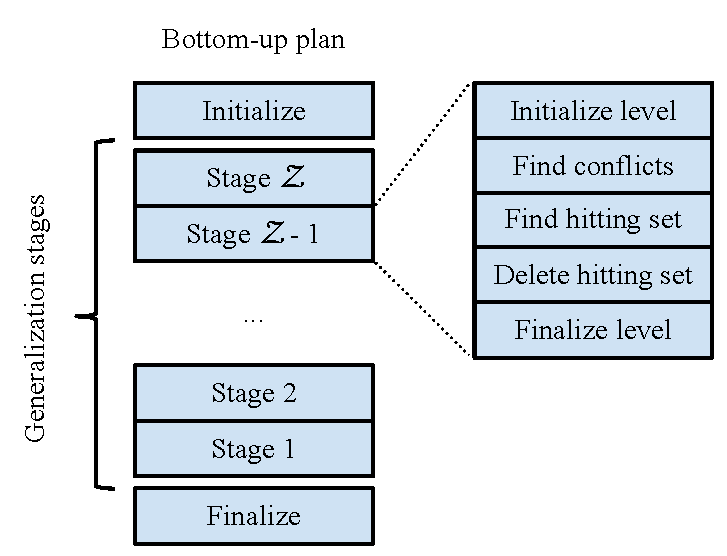
\includegraphics[scale=.6]{figs/cvl_stages.pdf}
\caption{The algorithmic framework: At stage $i$ the single-scale optimization problem is solved for the $i'th$ zoom level.}
\label{fig:algorithmic-framework}
\end{center}
\end{figure}

Below we describe three different heuristic algorithms for solving the single-scale optimization problem. Let $n=|C|$ be the number of constraints (or elements in the set multicover problem), and let $m=|R|$ be the number of records (or sets in the set multicover problem). Recall that $R_c \subseteq R$ is the set of records in constraint $c \in C$. The largest number of records in any constraint is $f = \max_{c \in C} |R_c|$, and is called the \emph{maximum frequency}.

\subsection{Static greedy algorithm (SGA)}

In this algorithm we consider each constraint $c \in C$ in turn, and simply choose the $\lambda_c$ records with minimum weight from constraint $R_c$ --- independently of what has been chosen earlier. If the sets $R_c$ are disjoint, the algorithm is clearly optimal. However, in general no approximation guarantee can be provided. The algorithm runs in $O(n f \log f)$ time, as we just need to sort the records by weight for each constraint; alternatively we can sort all records by weight in $O(m \log m)$ time and pick the minimum weight records from the constraints in linear time in the total number of records in all constraints.

\subsection{LP-based greedy algorithm (LPGA)}

In this algorithm we first solve a linear programming (LP) relaxation of the set multicover problem. This LP-problem is obtained by relaxing the constraint $x_r \in \{0, 1\}$ to $0 \leq x_r \leq 1$. Then we choose all records $r \in R$ for which the LP-solution variable $x_r$ is at least $\lambda_c / f$ (for some constraint $c \in C$ where $r \in R_c$). Intuitively, we round up all fractional values that are large enough. 

This algorithm provides a feasible solution to the single-scale problem, and the approximation guarantee is $\max_{c \in C} f / \lambda_c$~\cite{something}; thus, if $f$ is small, the algorithm provides a good approximation guarantee. As the LP-problem can be solved in polynomial time, the complete algorithm is polynomial.

\subsection{Dynamic greedy algorithm (DGA)}

Described in Vazirani 13.2.1. @Martin: Please write here.

\marcos{I would only introduce DGA if it is actually evaluated in the experiments.}

